\documentclass{report}

\usepackage{enumerate,fullpage,graphicx,hyperref}
\usepackage{tocloft}

\title{Emergent Architertural Design}
\date{Last edited: \today}
\author{Project members: \\
	\begin{tabular}{c c c}
	\hline 
		Derk-Jan Karrenbeld & 4021967 & 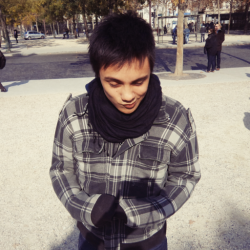
\includegraphics[scale=0.2]{../img/DJ.png}\\ 
		Joost Verdoorn & 1545396 & 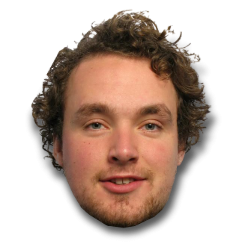
\includegraphics[scale=0.2]{../img/Yoloost.png}\\ 
		Steffan Sluis & 4088816 & 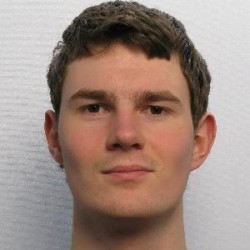
\includegraphics[scale=0.2]{../img/SS.jpeg}\\ 
		Tung Phan & 4004868 & 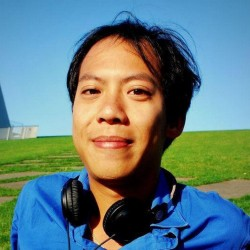
\includegraphics[scale=0.2]{../img/TP.jpeg}\\ 
		Vincent Robbemond & 4174097 & 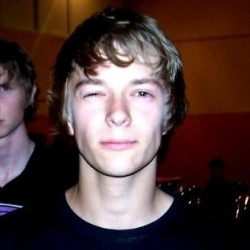
\includegraphics[scale=0.2]{../img/VR.jpeg}\\ 
		\hline 
	\end{tabular} 
	}

\begin{document}
	
	\maketitle

	\setcounter{section}{0}
	\setcounter{secnumdepth}{3}
	\setcounter{tocdepth}{5}
	\renewcommand*\thesection{\arabic{section}}
	
	\pdfbookmark{\contentsname}{toc}
	\tableofcontents

	\clearpage
	
	\section{Introduction}
		This document contains the architectural design for the application created during the Context Project `Programming Life: Synthetic Biology'. The application is targeted at synthetic biologists and its main purpose is to easily model, simulate and validate the complex workings of a cell. \\
		The design of this application is explained first in terms of its design goals. Then a subsystem decomposition follows, which serves to uncover the inner workings of the application, along with a description of the mapping of subsystems to processes and computers, a hardware/software mapping. After this, the management of data and shared resources is discussed. 
		\subsection{Design goals}
			The application can model cells and the processes within. The main design goal is to make this task as easy and intuitive as possible. Further, as requested by the client, it should:
			\begin{itemize}
				\item give an indication how changes to the cell will reflect on the rest of the cell
				\item have the ability to easily import and export datasets from and to frequently used data-formats e.g. CSV, SBML, HTML, PDF and Excel.
				\item give feedback to the user about mistakes and when possible provide a solution. An example is telling the user components are missing for a correctly working cell.
				\item compare simulations by plotting data on top of other simulations.
				\item be available offline, once the application is loaded once.
				\item have the functionality to share data with other users.
				\item have an easy way to undo changes.
			\end{itemize}
			To broaden their knowledge and expand their experience, the developers agreed to use programming languages and frameworks previously unknown to them.
	\clearpage
	\section{Architecture}
	
			\subsection{Overview}
				Because the application is available offline, the server-client relation is very decoupled. This means that the main functionality resides on the client. The server is merely used for administrative purposes, storing application and user data and providing the clientside functionality. A backend on the server also allows for data manipulation on the database.
				
			\subsection{Server}
				The primary function of the server is to provide the clientside application. After the application is downloaded the first time, it will reside on the client. Each time a client is online the application is automatically updated. \\
				The secondary function is to provide storage for everything created by the user. Sharing data is made possible by the storing functionality. \\
				In the figure below you can see this concept. The server provides all the client side assets and outputs these assets and html files to the client. The clients have a local copy of the database and can synchronise this with the server side database.
				\clearpage
				\begin{figure}[htb]
					\begin{center}
						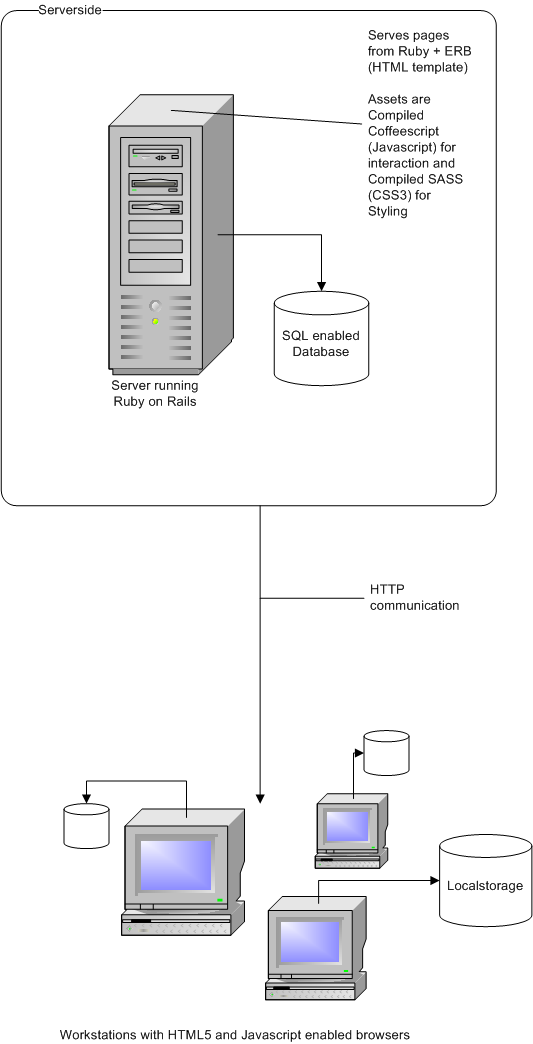
\includegraphics[height=20cm,keepaspectratio=true]{EAD.png}
						\caption{Deployment Diagram}
						\label{fig: EAD}
					\end{center}
				\end{figure}
				\clearpage
									
				\subsubsection{Rails}
					The server runs on Ruby on Rails \cite{ror} . This is a fairly new but very stable platform that is not only free but also open source. This means active development by a lot of people. Problems are easily fixed and this should ease the use of the application that is being designed. The language itself is written from a standpoint where you should just be able to write code and not worry about breaking the interpreter \cite{ruby} . This makes it easy to write comprehensible code that executes complex tasks.				
				\subsubsection{MVC on the server}
					The pages served are HTML5 for markup with CSS3 for styling and Javascript for interaction. Pages are built by a comprehensive and solid Model-Viewer-Controller system. This keeps data separated from the representation, further increasing maintainability. Interaction is illustrated in figure 3. Rails uses MVC in its core. It made it easy to create the backend views and client side representations because displaying data, the interaction and the actual data are seperated. This is a reason to stick with this system.
				\subsubsection{MVC Models and Database Design}
					\begin{figure}[htb]
						\begin{center}
							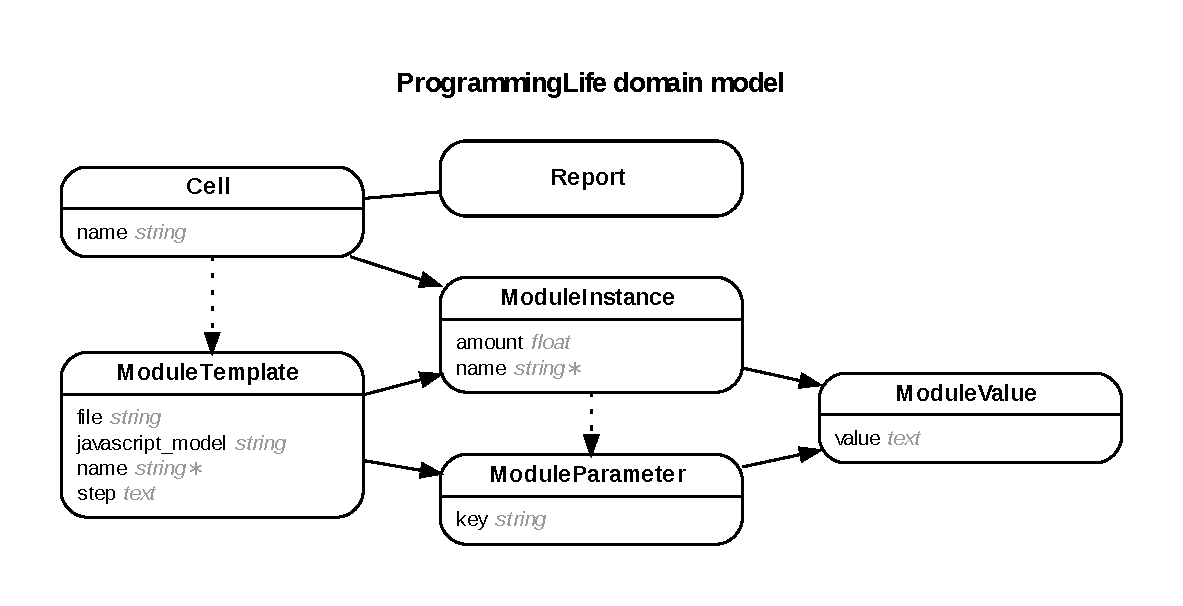
\includegraphics[width=\linewidth]{erd.pdf}
							\caption{Database and Ruby Models}
							\label{fig: erd}
						\end{center}
					\end{figure}	
					A report always shows the current cell data, so there is a one to one relation between reports and cells. The component definitions are seperated from the values. A cell contains components, called modules (module\_instance). These components are instances of blueprints (module\_template). Each component blueprint can provide multiple parameters (module\_parameter). Each instance has a value for each parameter (module\_value).\\
					The database design was devised this way, so templates are seperated from instances, resulting in no data redundancy.
				\subsubsection{Active Database}
					Ruby models are mapped to any Relational Database Management System (RDBMS \cite{rdbms} ) such as SQLite, MySQL and PostgreSQL. By not restricting the server database technology, switching systems, servers or extending their capacity should be fairly simple and easy. Database operations are done through Active Database, part of rails, which transparently maps the query to the technology's language.
				\subsubsection{Views and ERB} 
					The views are in ERB \cite{erb} which is an HTML template system. It comes with the Rails framework, so it does not require any extra software. Rails controllers written in Ruby can expose data to these views. Using a templating system such as this allows for quick translation from model to display. 
			\begin{figure}[htb]
				\begin{center}
				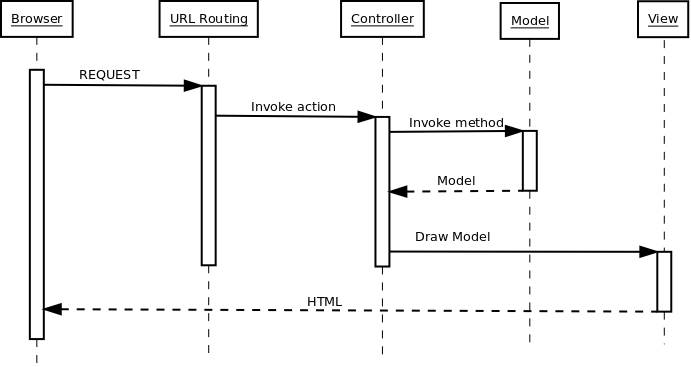
\includegraphics[width=\linewidth]{SequenceDiagramLife.png}
				\caption{Sequence Diagram}
				\label{fig: SequenceDiagram}
				\end{center}
				\end{figure}	
			\clearpage

			\subsection{Client}
				The server compiles the client application from Coffeescript to Javascript. This application is completely seperated from the server side functionality except for saving, loading, sharing and the production of reports. The client application is also built upon MVC.\\	
				
				\subsubsection{Models}
					\begin{figure}[htb]
						\begin{center}
							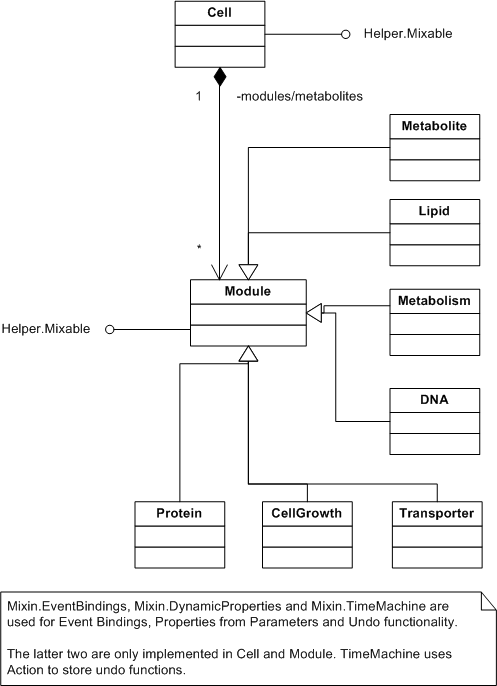
\includegraphics[width=\linewidth]{models.png}
							\caption{Client Models}
							\label{fig: cmodels}
						\end{center}
					\end{figure}	
					There are two data models and a few meta models. The cell has it's own model and so do the modules, cell components, such as transporters and metabolites. The JavaScript classes can be seen as the ModuleTemplate and ModuleParameter classes on the server. The contents of the classes, the actual data, are the ModuleInstance and ModuleValue classes. Each model has a bit of functionality but only
					to ensure data consistency and correctness. Each of these data models can load and save itself. \\
					To provide for undo functionality, the tree, node, undo tree and action classes are present. The former three are pretty transparent. The latter is a closure class used as node data in the tree. \\
					The Event Manager adds communication between arbitary part of the application. Objects can trigger events or listen on it.
				
				\subsubsection{Views}
					\begin{figure}[htb]
						\begin{center}
							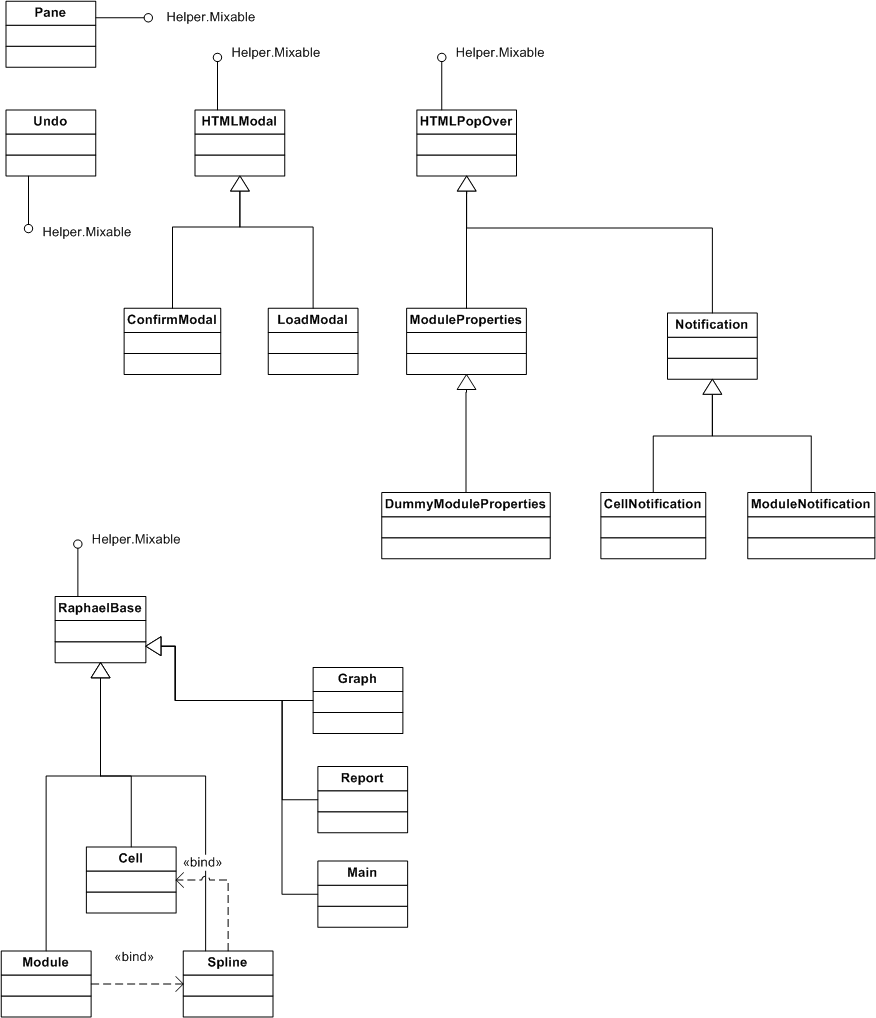
\includegraphics[scale=0.675]{views.png}
							\caption{Client Views}
							\label{fig: cmodels}
						\end{center}
					\end{figure}	

					The views are of two basic types: Raphael or HTML. There is a meta class Collection which just holds views. All views can have children and display a single model. Raphael typed views use SVG to display their contents. To display a model differently, new views can be added. The views only have display functionality. They do not add interaction. \\
					Events on the models ensure views to be able to update their display. This way a view is notified of changes instead of needing to poll for changes.
					
				\subsubsection{Controllers}
					\begin{figure}[htb]
						\begin{center}
							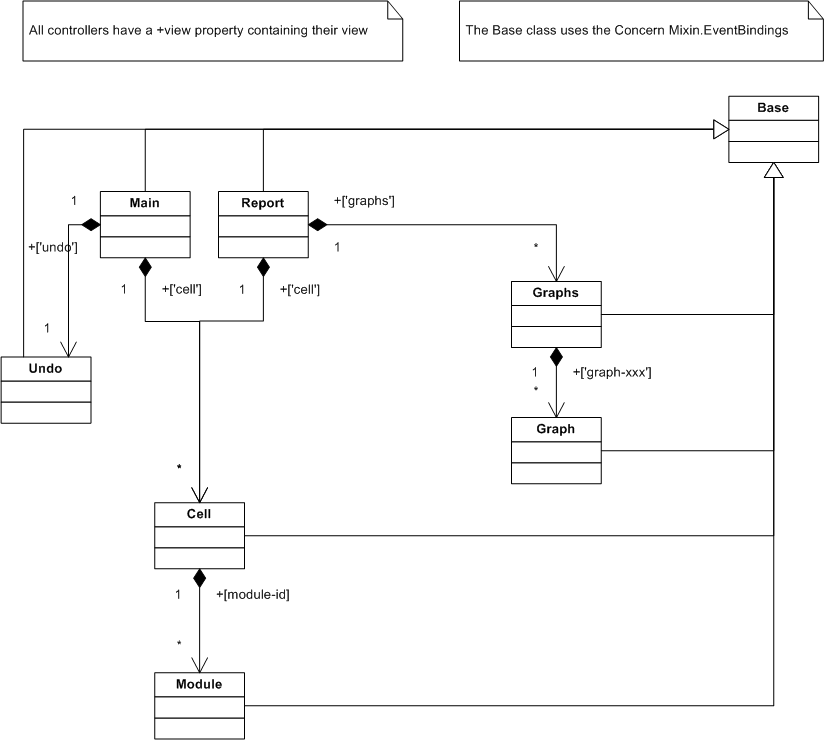
\includegraphics[width=\linewidth]{controllers.png}
							\caption{Client Controllers}
							\label{fig: cmodels}
						\end{center}
					\end{figure}	
					Controllers add interaction to views and models. Controllers can have children. Parent controllers can alter a child controllers behaviour. This way there is no need for a large set of controllers, e.g. a MainCell controller and a ReportCell are now combined into one Cell controller. \\
					For collections of elements, views can use unobtrusive JavaScript to enlist those elements for interaction. A view might add data-xxx attributes to elements. Controllers may or may not bind javascript to elements with these attributes. Keeps the HTML clean and the interaction in the controllers hand. 
				\clearpage
				\subsubsection{Helpers}
					\begin{figure}[htb]
						\begin{center}
							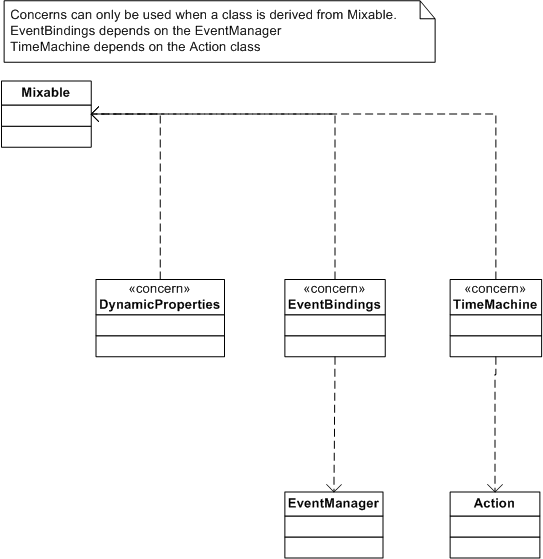
\includegraphics[width=\linewidth]{helpers.png}
							\caption{Client Helpers}
							\label{fig: cmodels}
						\end{center}
					\end{figure}	
					There is a set of mixins used by many models, views and controllers. DynamicProperties adds the ability to dynamically create javascript properties. Define getters, setters, non enumerable values and so forth and on. The Cell and Module models use this extensively. TimeMachine adds undo functionality to a class. EventBindings enable listening and triggering events, used by almost all classes. Catchable can enclose functions into try catch blocks and trigger callbacks and events instead of breaking the application. Finaly there is the Mixable base class. To use mixins, this class needs to be in the prototype chain.
					
				\subsubsection{Local storage}
					Javascript determines the local storage engine that is availabe and uses that to maintain an offline copy of the application and the created cells/modules. This makes it very easy to design new cells or edit saved cells even when the user isn't connected to the internet. This is communicated to the user, but requires no further interaction. Synchronization is completely transparent.
		
		\subsection{Data management}
			When the user has access to the server, it can export simulation results to a report in multiple standardised format, such as \emph{HTML}, \emph{Excel} and \emph{PDF} which can then be shared. Maintaining a standardised format allows for consistency in the reports as requested by the user.		
	
		\subsection{Concurrency}
			Each client runs independently and uses asynchronous communication with the server through \emph{REST}/\emph{CRUD} and \emph{AJAX}. Because of this, concurrency issues are very improbable. The client-side application is web-based, and uses only one process. Shared resources are retrieved atomically from and synchronised atomically with the database. Upon failure, the user is notified and possible solutions are provided. At this point the system does not allow concurrent edits on the same data, but this functionality was not requested by the user. Such functionality could be added in the future.\\		
			
	\clearpage
	\section{Software Technology}
		This section contains all the information about the software architecture of the application. The section is divided into several subsections to group together interesting information and improve readability.	
		
		\subsection{Framework and Development}
			This section describes the key technologies used during a release cycle.
			It is divided into three subsections; development, testing and production.
			The first subsection is about the development phase, where features are realised.
			The second section is about the testing phase, in which the features mentioned before are tested.
			The third section describes the production/release phase, in which a tested feature is implemented.
			
			\subsubsection{Development}
				During development we are making use of Coffeescript \cite{coffeescript} for writing interaction assets, SASS \cite{sass} for styling and SVG \cite{svg} with the Raphael \cite{raphael} framework for visualising part of the application.
				Coffeescript and SASS are preprocessors for respectively Javascript and CSS. Using these preprocessors gives us the advantage of cleaner syntax.
				By making use of SVG to render the cell every graphical object is also a DOM object, this enables us to attach Javascript event handlers and modify the objects itself.
				
			\subsubsection{Testing}
				We test the application in a Behaviour Driven Development (BDD \cite{bdd} ) and Test Driven Development (TDD \cite{tdd} ) way. 
				The Javascript assets are tested using the Jasmine framework \cite{jasmine} . 
				To run all tests in the browser we are making use of the Teabag framework \cite{teabag} . 
				To keep track of code coverage we are making use of the Istanbul framework \cite{istanbul} .
				The Ruby assets (database, MVC architecture - models, controllers, views - and Rails) are tested using the Rspec framework \cite{rspec} .  
				All tests run automatically using Continuous Integration, a practice in which tests are ran every time work has been done within critical sections of the code. 
				Tests and coverage are used to ensure maintainability, consistency and quality of the code.
				
			\subsubsection{Release}
				During the Production release the Coffeescript assets are compiled to Javascript \cite{javascript} and the SASS assets are compiled to CSS, after which they are minified and bundled using uglifier \cite{uglifier} . Minified assets take up less space and increase page performance which results in a better user experience and less demand on the web server. 
				SVG is still used for creating visualisations of the cell models.
		\newpage		
		\subsection{Ordinary Differential Equation Solver}
			All computations run client-side and are performed by our ODE Solver, which is built upon the numericjs \cite{numericjs} library. This is a library which makes it possible to perform sophisticated numerical computations in pure JavaScript and thus is able to run in the browser. The ODEs are solved using the Dormand-Prince RK method \cite{dormandprince} , also known as the ode45-function in MATLAB (previously used by our client).
			
		\subsection{API}
			The API can be found online here: \url{http://coffeedoc.info/github/Derkje-J/programming-life/} \\
			In the future there will be a Rubydoc online for server-side assets and is updated after each commit.
		\newpage
			
	\section{Summary}
		The application is a lightweight, cross-platform graphical design tool with a centralised storage database. The architecture ensures its functionality on different kinds of machines as well as the ease of simulating complex cell models. It not only offers stability, ease and intuitive design, it offers it on every modern machine. During development of this application the design goals are continuously used as a mandate for the functionality and dictates the production flow.
	\section{Glossary}
		This section explains any and all terms that may be ambiguous or unclear:\\
		
		\textbf{REST}: Representational State Transfer, or REST, is an architectural style of large-scale networked software that takes advantage of the technologies and protocols of the World Wide Web. \\
See \href{http://goo.gl/Lfwhs}{http://goo.gl/Lfwhs} for more information.

\clearpage

\begin{thebibliography}{9}

\bibitem{ror}
Ruby on Rails,
\emph{A web-application framework to create database-backed web applications according to the Model-View-Controller (MVC) architecture.}
\href{http://api.rubyonrails.org/}{http://api.rubyonrails.org/}

\bibitem{ruby}
Bill Venners,
\emph{The Philosophy of Ruby}.
2003.
\href{http://www.artima.com/intv/rubyP.html}{http://www.artima.com/intv/rubyP.html}

\bibitem{rdbms}
Relational Database Management System, 
\emph{a database management system that is based on the relational model.}
\href{http://en.wikipedia.org/wiki/Relational\_database\_management\_system}{http://en.wikipedia.org/wiki/Relational\_database\_management\_system}

\bibitem{erb}
ERB,
\emph{a simple but powerful templating system.}
\href{http://ruby-doc.org/stdlib-2.0/libdoc/erb/rdoc/ERB.html}{http://ruby-doc.org/stdlib-2.0/libdoc/erb/rdoc/ERB.html}

\bibitem{coffeescript}
Coffeescript,
\emph{a language that compiles into JavaScript.}
\href{http://coffeescript.org/\#language}{http://coffeescript.org/\#language}

\bibitem{sass}
SASS,
\emph{ an extension of CSS3.}
\href{http://sass-lang.com/docs/yardoc/file.SASS\_REFERENCE.html}{http://sass-lang.com/docs/yardoc/file.SASS\_REFERENCE.html}

\bibitem{svg}
SVG,
\emph{an XML-based vector image format for two-dimensional graphics that has support for interactivity and animation.}
\href{http://www.w3.org/Graphics/SVG/}{http://www.w3.org/Graphics/SVG/}

\bibitem{raphael}
Raphael,
\emph{a JavaScript library that should simplify working with vector graphics on the web.}
\href{http://raphaeljs.com/reference.html}{http://raphaeljs.com/reference.html}

\bibitem{bdd}
Behaviour Driven Development,
\emph{a software development process based on test-driven development (TDD).}
\href{http://en.wikipedia.org/wiki/Behavior\-driven\_development}{http://en.wikipedia.org/wiki/Behavior\-driven\_development}

\bibitem{tdd}
Test Driven Development,
\emph{a software development process where tests are written first}
\href{http://en.wikipedia.org/wiki/Test\-driven\_development}{http://en.wikipedia.org/wiki/Test\-driven\_development}

\bibitem{jasmine}
Jasmine,
\emph{a behavior-driven development framework for testing JavaScript code.}
\href{http://pivotal.github.io/jasmine/}{http://pivotal.github.io/jasmine/}

\bibitem{teabag}
Teabag,
\emph{ a Javascript test runner built on top of Rails.}
\href{https://github.com/modeset/teabag}{https://github.com/modeset/teabag}

\bibitem{istanbul}
Istanbul,
\emph{a Javascript code coverage tool written in Javascript.}
\href{https://github.com/gotwarlost/istanbul}{https://github.com/gotwarlost/istanbul}

\bibitem{rspec}
Rspec framework,
\href{http://rubydoc.info/gems/rspec\-rails/frames}{http://rubydoc.info/gems/rspec\-rails/frames}

\bibitem{javascript}
Javascript
\href{https://developer.mozilla.org/en-US/docs/JavaScript/Reference}{https://developer.mozilla.org/en-US/docs/JavaScript/Reference}

\bibitem{uglifier}
Uglifier,
\emph{Ruby wrapper for UglifyJS JavaScript compressor.}
\href{http://rubydoc.info/gems/uglifier/2.1.0/frames}{http://rubydoc.info/gems/uglifier/2.1.0/frames}

\bibitem{numericjs}
NumericJS,
\emph{a library which allows you to perform sophisticated numerical computations in pure javascript in the browser and elsewhere.}
\href{http://www.numericjs.com/}{http://www.numericjs.com/}

\bibitem{dormandprince}
Dormand-Prince RK method ,
\emph{a method for solving ordinary differential equations.}
\href{http://en.wikipedia.org/wiki/Dormand\%E2\%80\%93Prince\_method}{http://en.wikipedia.org/wiki/Dormand\%E2\%80\%93Prince\_method}

\end{thebibliography}

\end{document}
